\chapter{Caracterización de ataques a ICS con Mitre}
\label{chap:01}
\section*{Introducción}

La tarea nos pide de leer un artículo de revisión de 15 ataques a sistemas de control industrial (ICS) y elegir 5 de ellos para caracterizarlos con la matriz de \href{attack.mitre.org/matrices/ics/}{Mitre ATT\&CK}. La matriz de Mitre ATT\&CK es una base de datos de tácticas, técnicas y procedimientos (TTP) utilizados por los atacantes en el ciberespacio. Esta matriz se utiliza para comprender mejor las amenazas y mejorar la defensa cibernética.

\framedt{Tarea a realizar}{
\begin{itemize}
	\item Lee detenidamente el documento para reforzar los conceptos expuestos en clase sobre seguridad en ICS e infraestructuras críticas.
	\item Elige los 5 ataques que consideres más significativos o que pienses que están mejor descritos.
	\item Para cada uno de esos ataques,  en base a la información del documento, y al contenido de la matriz de MITRE para ICS,  indica que tácticas y técnicas  utilizaron los atacantes. Explica porqué piensas que en cada caso utilizaron esas tácticas y técnicas. Indica también el tipo de respuesta descrito para cada ataque y si te parece adecuado, o bien propondrías otro tipo posible de respuesta.
\end{itemize}
}

\subsection{WWS and ICSs}

El artículo empieza con una introducción sobre el WWS (Water and Wastewater Sector), que es un sector crítico para la sociedad, ya que proporciona agua potable y trata las aguas residuales. 
Este es, según el U.S. Department of Homeland Security, uno de los sectores más targetados por los ciberataques. Su salvaguardia frente a las amenazas de ciberseguridad se considera una cuestión de prioridad nacional.

WWS son sistemas de control industrial (ICS) que se utilizan para supervisar y controlar las infraestructuras de agua y aguas residuales. Estos sistemas son esenciales para garantizar la calidad del agua, la eficiencia operativa y la seguridad pública.

La major parte de los ICS en el sector WWS son sistemas SCADA (Supervisory Control and Data Acquisition), que permiten la supervisión y control remoto de los procesos industriales. Estos sistemas se componen de sensores, controladores lógicos programables (PLC) y estaciones de trabajo que se comunican entre sí para supervisar y controlar los procesos.

Hay una MTU (Master Terminal Unit) que se encarga de la supervisión y control de los procesos, y una RTU (Remote Terminal Unit) que se encarga de la supervisión y control de los dispositivos remotos. La MTU se comunica con la RTU a través de una red de comunicación, que puede ser una red privada o una red pública.
La HMI (Human-Machine Interface) es la interfaz que permite a los operadores interactuar con el sistema SCADA. La HMI se utiliza para supervisar y controlar los procesos, y para visualizar la información del sistema.

Durante muchos años, los sistemas SCADA y, en general, las redes OT en entornos industriales, estaban
no estaban conectadas a las redes informáticas corporativas ni a Internet. Sin embargo, a medida que la tecnología avanzaba, muchas organizaciones planearon consolidar las redes IT y OT superpuestas.

\subsection{Redes ICS}

La nueva generación de redes IT-OT convergentes en los sistemas de control industrial, también conocida como Industrial Internet of Things (IIoT), ya no está air-gapped.\\
Una red ICS està dividida por niveles y zonas:
\begin{itemize}
   \item \textbf{Enterprise zone }- that includes assets for business logistics and enterprise systems, representing Level 4 and 5, respectively. This zone is also known as IT network.
   \item \textbf{Demilitarized zone (DMZ) }- that separates IT and OT networks, thus preventing direct access to OT devices from the IT network. All corporate-accessible services (e.g., web, 120 email) reside in this zone
   \item \textbf{Manufacturing and Control zone }- The former refers to the entire OT domain, including Levels 0, 1, 2, and 3; the latter refers to Levels 0, 1, and 2, so it is equivalent to the traditional ICS architecture shown in Figure 1a. Level 3 provides site-level operation and asset management. Plant historian, production scheduling and reporting, patch and file services reside at Level 3
\end{itemize}

\subsection{Ataques a ICS}
Los ataques a sistemas de control industrial (ICS) son cada vez más frecuentes y sofisticados. En este trabajo, analizaremos cinco ataques significativos a sistemas de agua y aguas residuales (WWS), utilizando la matriz de MITRE ATT\&CK para ICS. Esta matriz nos permite categorizar las tácticas, técnicas y procedimientos utilizados por los atacantes en entornos ICS.

Vamos a analizar las tácticas y técnicas utilizadas en cada ataque, así como la respuesta a los incidentes y su efectividad.
\newpage
\section{Ataque 1: Maroochy Water Services, Australia, 2000}

\subsection{Descripción del incidente}
En el año 2000, un ex empleado atacó el sistema SCADA de Maroochy Shire en Queensland, Australia. El atacante era un antiguo supervisor de sitio para Hunter Watertech Pty Ltd (HWT), un contratista externo que había instalado RTUs en 142 estaciones de bombeo. Después de renunciar en diciembre de 1999, realizó múltiples intrusiones al sistema SCADA entre enero y abril del 2000, causando malfuncionamientos como pérdida de comunicaciones, falsas alarmas y alteración de configuraciones. El resultado fue la liberación de aproximadamente un millón de litros de aguas residuales sin tratar al medio ambiente.
\nl

\coolquote{
    The main hazard involved in this incident was the unauthorized access to the SCADA system, which enabled the malevolent actor to release raw sewage into the surrounding environment. There were no cybersecurity procedures, policies, or defenses present, and the service contract was deficient or inadequate to handle the contractor’s responsibilities.
}{}
\nl

\subsection{Tácticas y técnicas según MITRE ATT\&CK}
Según la matriz MITRE ATT\&CK para ICS, el ataque utilizó las siguientes tácticas y técnicas:

\begin{itemize}
    \item \textbf{Initial Access} - El atacante utilizó la técnica de \textit{Use of Valid Credentials} (T0859), ya que mantuvo acceso a sus credenciales después de dejar la empresa.\\
    T0859 aparece en la sección \textit{Persistence} de la matriz MITRE ATT\&CK para ICS, pero claro que se puede utilizar también para el acceso inicial.\\
    La falta de procedimientos para revocar accesos de exempleados facilitó su intrusión y persistencia en el sistema durante meses.
    
    
    \item \textbf{Execution} - Empleó la técnica de \textit{Execution through API} (T0871), utilizando su conocimiento para enviar comandos legítimos con intenciones maliciosas.\\
    Siendo un ex supervisor, tenía un conocimiento profundo del sistema y su funcionamento. Esto le permitió emitir comandos de ingeniería que parecían legítimos pero causaban daños significativos.
    
    \item \textbf{Impact} - Utilizó la técnica de \textit{Modify Parameter} (T0836), alterando la configuración de las estaciones de bombeo para causar el vertido de aguas residuales.\\
    También utilizó la técnica de \textit{Loss of Safety} (T0880), desactivando exitosamente las alarmas de cuatro bombas.\\
    La manipulación de parámetros de control fue una táctica efectiva dada la ausencia de monitoreo de comportamientos anómalos en el sistema.
\end{itemize}

% \subsubsection{Justificación de las tácticas y técnicas}
% El atacante eligió estas tácticas y técnicas por varias razones:

% \begin{itemize}
%     \item Como ex supervisor del proyecto, tenía un conocimiento íntimo del sistema y sus vulnerabilidades, lo que le permitió aprovechar credenciales válidas para acceder al sistema.
    
%     \item La falta de procedimientos para revocar accesos de exempleados facilitó su intrusión y persistencia en el sistema durante meses.
    
%     \item Su conocimiento técnico le permitió emitir comandos de ingeniería que parecían legítimos pero causaban daños significativos.
    
%     \item La manipulación de parámetros de control fue una táctica efectiva dada la ausencia de monitoreo de comportamientos anómalos en el sistema.
% \end{itemize}

\begin{figure}[htbp]
    \centering
    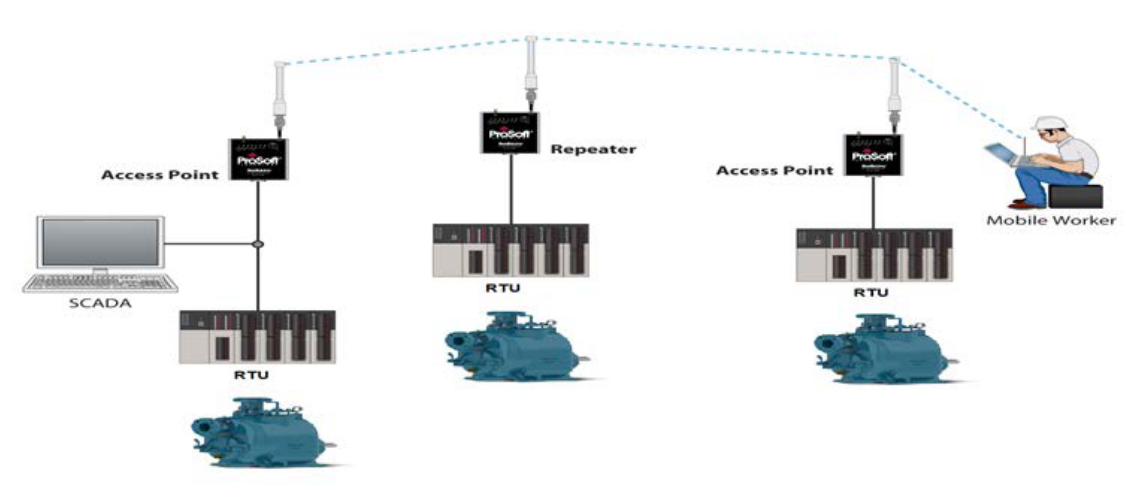
\includegraphics{images/maroochyScada.png}
    \caption{Cómo funcionarían el SCADA de Maroochy y la RTU (Unidad Terminal Remota)}
    \label{fig:maroochyScada}
\end{figure}


\newpage

\subsection{Respuesta al incidente}
La respuesta consistió en una investigación que culminó con la captura del sospechoso en abril de 2000. Se le encontró en posesión de equipos de control industrial, como un ordenador Compact 500, un radio bidireccional, un portátil, un transformador y cables. Posteriormente fue sentenciado a dos años de prisión y ordenado a pagar 13,111 dólares australianos por los daños causados. La limpieza del vertido requirió días y recursos sustanciales.

\subsubsection{Evaluación de la respuesta}

\begin{paracol}{2}
    \colfill
    
    La respuesta fue reactiva y no preventiva. Como se sugiere en el artículo, la respuesta parece inadecuada por varias razones:
    
    \begin{itemize}
        \item No existían procedimientos de ciberseguridad que pudieran prevenir el ataque.
        \item No había un sistema para revocar accesos cuando un empleado dejaba la empresa.
        \item Tardaron mucho tiempo en identificar que las fallas eran causadas por intervención humana.
    \end{itemize}
    
    Una respuesta más adecuada habría incluido la implementación de controles de seguridad básicos según el protocolo NIST SP 800-53, como la terminación inmediata de accesos de exempleados, autenticación multifactor, segregación de redes y monitoreo continuo de actividades sospechosas en el sistema SCADA.
    \colfill

    \switchcolumn

    \begin{figure}[htbp]
        \centering
            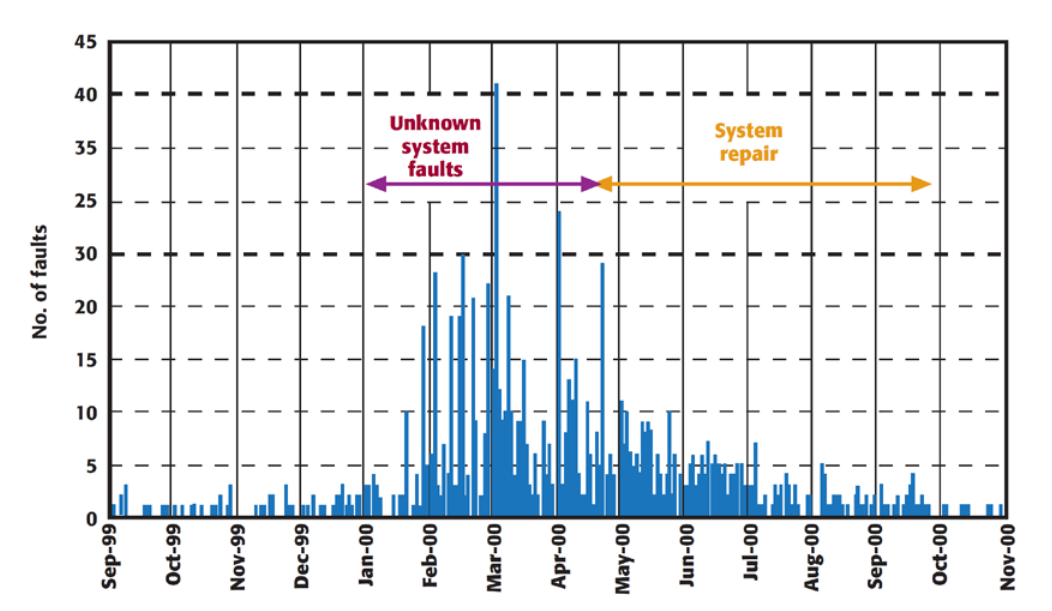
\includegraphics[width=1\columnwidth]{images/maroochyFaults.png}
            \caption{Número de fallas en el sistema SCADA de Maroochy Shire, antes y después del incidente}
            \label{fig:maroochyFaults}

            Parece interesante ver que el número de fallas tomó bastante tiempo después del último ataque el 23 de abril para volver a valores normales.
    \end{figure}

\end{paracol}



Bloquear el \textbf{acceso inicial} a los atancates es fundamental. Constituye la primera línea de defensa contra ataques a ICS y a sistemas informaticos en general. Tras obtener acceso, los atacantes pueden escanear la red, detectar vulnerabilidades, moverse lateralmente y comprometer sistemas críticos.

Además, la falta de ciberconciencia situacional, es decir, la falta de conocimiento sobre lo que está sucediendo en el sistema, no ha permitido de detectar sin demora el ataque.\\
Además de la falta de ciberconciencia situacional, parece evidente que faltaba la definición clara de políticas de \textbf{Access Control}, que es fundamental y que tiene que funcionar como guía para la implementación y configuración de las herramientas de seguridad.\\
Un firewall, sin una política de acceso bien definida, no es más que un filtro que pero no puede resolver ningún problema concreto de seguridad.
\newpage


\section{Ataque 2: Kemuri Water Company (seudónimo), EE.UU., 2016}

\subsection{Descripción del incidente}
\begin{paracol}{2}
    \colfill
    En 2016, una empresa de servicios de agua en EE.UU. (bajo el seudónimo Kemuri Water Company) contrató a Verizon Security Solutions para realizar una evaluación de ciberseguridad de sus sistemas. La evaluación reveló vulnerabilidades de alto riesgo, incluyendo el uso de sistemas obsoletos como un ordenador \href{https://it.wikipedia.org/wiki/IBM_AS/400}{AS400} que servía para funciones críticas de IT y OT, con conexiones directas a múltiples redes. El análisis forense descubrió que hacktivistas patrocinados por un estado habían explotado la aplicación de pago en internet para acceder al sistema AS400, resultando en la exfiltración de 2.5 millones de registros únicos y manipulación de productos químicos y tasas de flujo.
    \colfill
    
    \switchcolumn

    \begin{figure}[htbp]
        \centering
        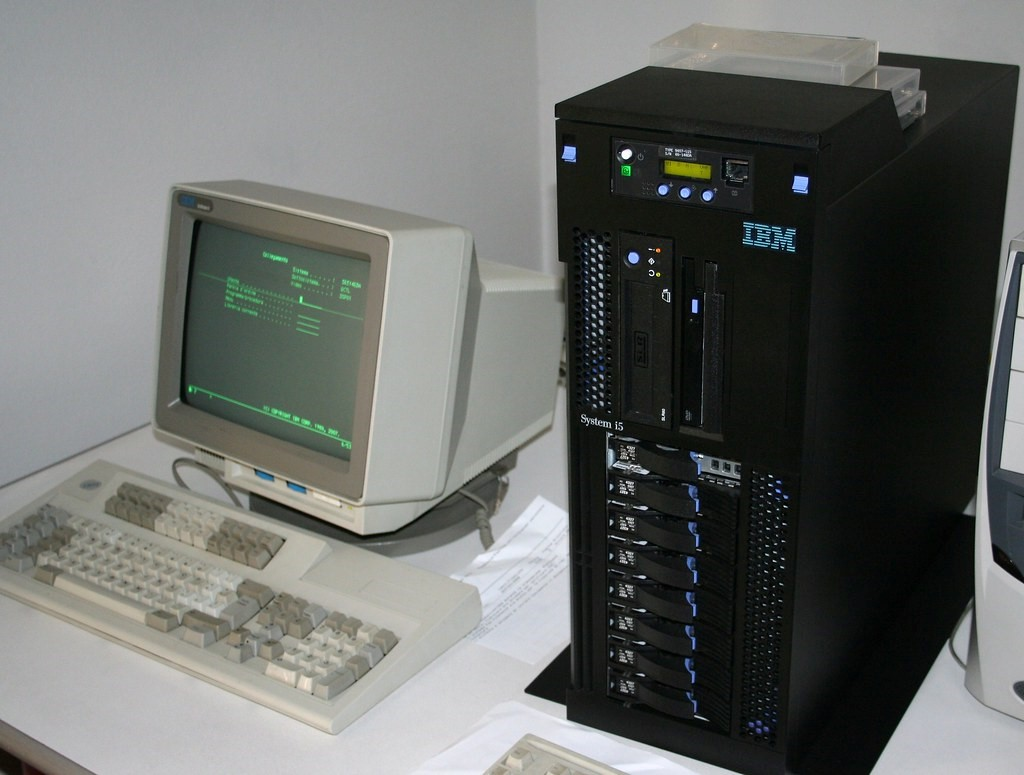
\includegraphics[width=0.95\columnwidth]{images/AS400.jpg}
        \caption{AS400 IBM}
        \label{fig:AS400}
    \end{figure}
\end{paracol}


\subsection{Tácticas y técnicas según MITRE ATT\&CK}

\begin{paracol}{2}

    \colfill
    \begin{figure}[htbp]
        \centering
        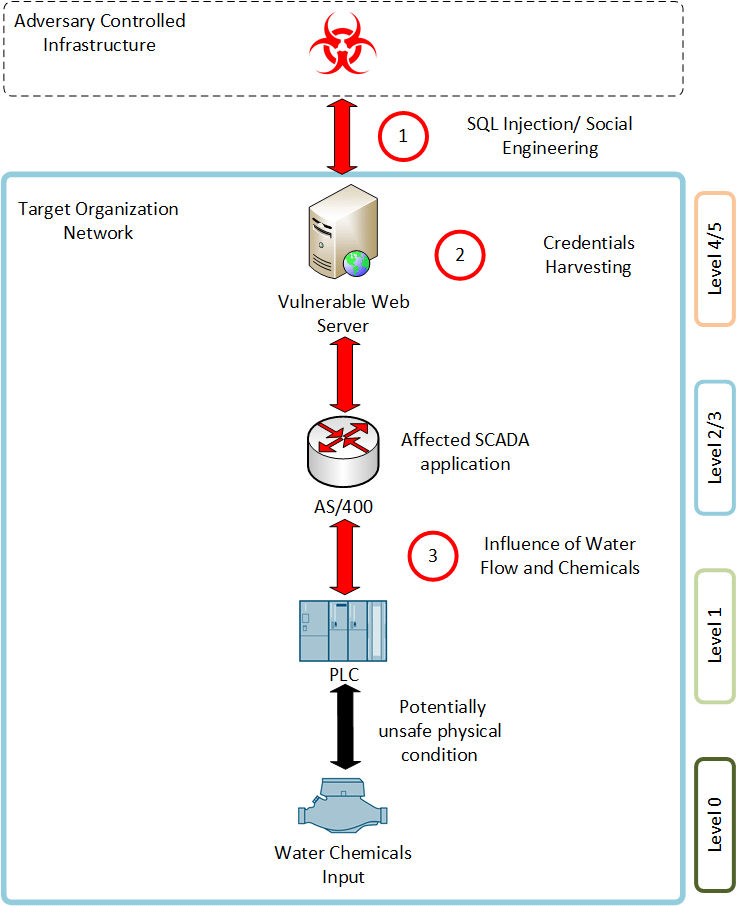
\includegraphics[width=1\columnwidth]{images/kemuri.png}
        \caption{Kemuri attack diagram}
        \label{fig:kemuri}
    \end{figure}
    \colfill

    \switchcolumn
    \colfill



Según la matriz MITRE, este ataque empleó:

\begin{itemize}
    \item \textbf{Initial Access} - \textit{Exploit Public-Facing Application} (T0819), aprovechando vulnerabilidades en la aplicación de pago por internet.
    Esto permitió a los atacantes obtener acceso inicial al sistema IT, que estaba conectado directamente al sistema OT (AS400).
    
    % \item \textbf{Lateral Movement} - \textit{Exploitation of Trust Relationships} (T0884), utilizando la conexión entre la aplicación de pago y el sistema AS400.
    
    \item \textbf{Collection} - \textit{Automated Collection} (T0802), obteniendo información sobre el sistema de control industrial.
    
    \item \textbf{Impact} - \textit{Modify Parameter} (T0836), alterando productos químicos y tasas de flujo.
\end{itemize}

\subsubsection{Justificación de las tácticas y técnicas}
Los atacantes eligieron estas tácticas porque:

\begin{itemize}
    \item La aplicación de pago por internet presentaba una puerta de entrada fácil al no estar adecuadamente protegida.
    
    \item La conexión directa entre el sistema IT (aplicación de pago) y OT (AS400) representaba una ruta de confianza que eliminaba la necesidad de superar barreras adicionales de seguridad.
    
    \item El sistema AS400 obsoleto carecía de parches de seguridad y controles modernos, facilitando la recolección de datos y manipulación de parámetros.
    
    \item La autenticación de factor único simplificó el acceso no autorizado a sistemas críticos.
\end{itemize}
    \colfill
\end{paracol}


\subsection{Respuesta al incidente}
% Internet-facing servers and applications, such the
% 453 payment management application here, should not be connected to the SCADA
% The utility had
% 454 relied on a single-factor authentication; this is not sufficient, and multi-factor authentication should
% 455 be used. Outdated systems, like the AS400 here, which formed a single point of failure, should not
% 456 be deployed, and installation of security patches should not be overlooked.

La respuesta incluyó la terminación inmediata del acceso hacia y desde el sistema de gestión de cuentas web y el bloqueo de la conectividad saliente del sistema AS400. Se recomendó reemplazar los sistemas antiguos con versiones más modernas.

Lo que parece extraño es que algunos empleados sabían de las vulnerabilidades del sistema, y por lo tanto existe una duda sobre si la investigación requerida fue en realidad proactiva o reactiva.

\subsubsection{Evaluación de la respuesta}
La respuesta parece adecuada porque reveló adecuadamente las vulnerabilidades y llevó a la identificación del vector de ataque. Sin embargo, parece ser principalmente reactiva y carece de la implementación de medidas preventivas fuertes inmediatas.

Algunas ídeas de mejora serían:
\begin{itemize}
    \item Implementación de arquitectura de segmentación de red con zonas desmilitarizadas (DMZ) entre IT y OT.
    \item Autenticación multifactor para todos los sistemas críticos.
    \item Monitoreo continuo de tráfico de red entre zonas IT y OT.
    \item Evaluaciones periódicas de vulnerabilidades y pruebas de penetración.
\end{itemize}

Si hubiera habido un control periódico y mayor monitoreo, las vulnerabilidades habrían sido identificadas antes, y ---esperablemente--- el ataque habría sido prevenido.\\
Además, el hecho de que algunos empleados conocían vulnerabilidades denota negligencia y/o falta de comunicación entre equipos.\\
La falta de comunicación y un monitoring deficiente evidentemente contribuyeron a una \textit{``Ciberconciencia situacional''} parcial, es decir, que no se sabía lo que estaba pasando en el sistema. Hemos visto en clase que, herramientas de Visualización o una COP (Common Operational Picture) pueden ayudar a mejorar la comunicación entre los equipos y a obtener una vista general más completa.
En cualquier caso, es importante recalcar nuevamente que un sistema de filtrado o de autenticación para hacer segura una aplicación de cara al público por sí solos no son suficientes, es necesario definir reglas de acceso y autorización claras y eficaces, para que tales herramientas puedan efectivamente proteger el sistema.
\newpage
\section{Ataque 3: Empresa de agua europea, 2018}

\subsection{Descripción del incidente}
En enero de 2018, una empresa europea de servicios de agua con un sistema de análisis OT basado en la nube contrató a Radiflow para monitorear su red. El 21 de enero, se detectó tráfico de red sospechoso en la red SCADA, con nuevos enlaces a direcciones IP externas que generaban un cambio importante en la topología de la red. La investigación reveló que las direcciones pertenecían a un ``MinerCircle Monero Pool", lo que llevó a la detección de malware de criptominería en la red OT. Aproximadamente el 40\% del tráfico estaba relacionado con operaciones de minería, causando un aumento del 60\% en el consumo total de ancho de banda. Este incidente se considera el primer caso conocido de ``\textbf{cryptojacking}" contra un sistema ICS.

\begin{figure}[htbp]
    \centering
    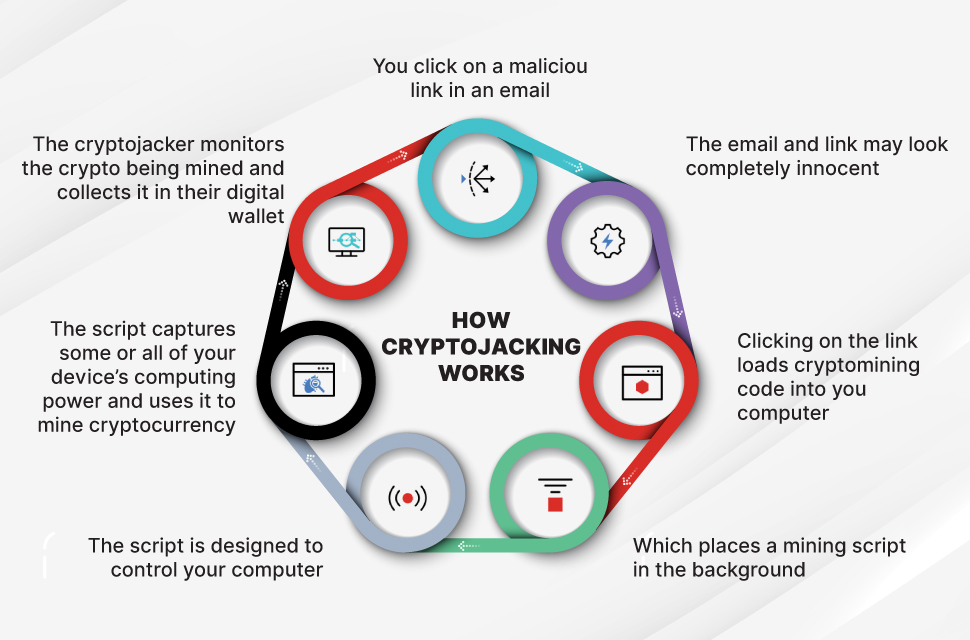
\includegraphics[width=0.85\columnwidth]{images/cryptojacking.jpg}
    \caption{Cryptojacking esquema}
    \label{fig:cryptojacking}
\end{figure}

\subsection{Tácticas y técnicas según MITRE ATT\&CK}
Las tácticas y técnicas utilizadas incluyen:

\begin{itemize}
    \item \textbf{Initial Access} - Aunque no se especifica en el documento, probablemente utilizaron \textit{Exploit Public-Facing Application} (T0819). De lo contrario, un empleado podría haber sido el culpable, o bien víctima de phishing (\textit{Spearphishing Attachment} T0865).

        \item \textbf{Execution} - \textit{Scripting} (T0853), ejecutando scripts maliciosos para la minería de criptomonedas.
        
        \item \textbf{Impact} - \textit{Resource Hijacking}\footnote{Esta es la técnica \href{https://attack.mitre.org/techniques/T1496/}{T1496}, mencionada en la categoria \textit{Enterprise}, no \textit{ICS}; sin embargo si puede considerar relacionada a la \href{https://attack.mitre.org/techniques/T0826/}{T0826}} (/\textit{Loss of Availability} T0826), utilizando recursos computacionales del sistema para minar criptomonedas.\\
        No hay exactamente la intención de causar daño directo a los activos, sino de aprovechar sus recursos para beneficio económico del atacante.
        Sin embargo, el resultado es un mayor consumo de recursos y uso de ancho de banda, lo que puede llevar a degradación del rendimiento y potencial denegación de servicio para operaciones legítimas.
\end{itemize}

\subsubsection{Justificación de las tácticas y técnicas}
Los atacantes eligieron estas tácticas por:

\begin{itemize}
    % \item Los sistemas OT basados en la nube ofrecen superficies de ataque que pueden no estar adecuadamente protegidas, permitiendo el acceso inicial.
    
    \item El malware de criptominería es relativamente fácil de implementar y puede pasar desapercibido durante períodos prolongados si no se monitorea adecuadamente el rendimiento del sistema.
    
    \item A diferencia de ataques que buscan interrumpir servicios o robar datos, el cryptojacking busca mantenerse operativo el mayor tiempo posible para maximizar ganancias.
    
    \item Los sistemas ICS suelen tener capacidad computacional constante y conexión permanente a internet, lo que los convierte en objetivos atractivos para la minería de criptomonedas.

\end{itemize}

\subsection{Respuesta al incidente}
La empresa de seguridad informó a la empresa de agua sobre el malware de criptominería y los servidores infectados. La recuperación incluyó la actualización del software antivirus en algunos servidores y el refuerzo de la seguridad del firewall. El software antivirus actualizado tuvo éxito en detectar el malware CoinMiner.

\subsubsection{Evaluación de la respuesta}
La respuesta fue adecuada pero reactiva.\\
La detección temprana del tráfico sospechoso permitió mitigar el impacto.
La actualización de antivirus y refuerzo de firewalls fueron medidas apropiadas, que deberían ayudar a prevenir incidentes similares en el futuro.

Para fortalecer un ICS contra ataques similares, propondría adicionalmente:
\begin{itemize}
    \item Implementación de sistemas de monitoreo de rendimiento para detectar anormalidades en el uso de recursos.\\
        Para ICSs, el tráfico y uso de recursos son a menudo predecibles, por lo que un valor anómalo en el uso de CPU o ancho de banda puede indicar actividad maliciosa, y se puede fácilmente detectar.
        \item Segmentación de red más estricta entre sistemas OT y conexiones externas.
        Esto se puede combinar con auditorías regulares de tráfico de red para identificar comunicaciones sospechosas, que de alguna manera se desvían de los patrones previstos.
        \item Implementación de listas blancas de aplicaciones para prevenir la ejecución de software no autorizado.
        Para una empresa de distribución de agua esto no debería ser demasiado difícil de implementar y mantener actualizado.
\end{itemize}

Hay técnicas de active/passive fingerprinting para establecer un perfil de tráfico normal, que pueden ayudar a detectar anomalías en el tráfico de red.\\
Sin embargo, un utilizo continuo de tecnicas de active fingerprinting pueden causar problemas de rendimiento y disponibilidad, que en un ICS pueden ser críticos.




% \section{Ataque 4: Onslow Water and Sewer Authority, EE.UU., 2018}

% \subsection{Descripción del incidente}
% En octubre de 2018, Onslow Water and Sewer Authority, una empresa de servicios de agua en Jacksonville (Carolina del Norte), fue atacada por ciberdelincuentes justo después del Huracán Florence. El ataque comenzó con ataques persistentes a través de un virus conocido como EMOTET. Mientras se investigaba, aproximadamente a las 3 am de un sábado, el malware lanzó un virus más sofisticado llamado RYUK, que encriptó archivos y datos. El equipo de IT desconectó inmediatamente las instalaciones de internet, pero no pudieron evitar el cifrado. Los atacantes enviaron un correo electrónico exigiendo un pago para descifrar los archivos dañados, pero la autoridad rechazó negociar.

% \subsection{Tácticas y técnicas según MITRE ATT\&CK}
% El ataque utilizó las siguientes tácticas y técnicas:

% \begin{itemize}
%     \item \textbf{Initial Access} - \textit{Spearphishing Attachment} (T0865), probablemente utilizando EMOTET para el acceso inicial.
    
%     \item \textbf{Persistence} - \textit{Project File Infection} (T0873), asegurando que EMOTET permaneciera activo en el sistema.
    
%     % \item \textbf{Execution} - \textit{User Execution} (T0863), desplegando el ransomware RYUK en un momento estratégico.
    
%     \item \textbf{Impact} - \textit{Data Manipulation} (T0831), cifrando datos críticos para exigir rescate.
% \end{itemize}

% \subsubsection{Justificación de las tácticas y técnicas}
% Los atacantes eligieron estas tácticas porque:

% \begin{itemize}
%     \item El momento después de un desastre natural (Huracán Florence) representaba un período de vulnerabilidad aumentada, con personal posiblemente distraído por tareas de recuperación.
    
%     \item El lanzamiento del ransomware RYUK a las 3 am de un sábado fue estratégico para minimizar la posibilidad de respuesta inmediata.
    
%     \item La combinación de EMOTET (para acceso inicial) y RYUK (para el cifrado) representa un ataque en dos etapas que dificulta la detección y respuesta.
    
%     \item El objetivo era claramente financiero, utilizando el cifrado de datos críticos como mecanismo de presión para el pago del rescate.
% \end{itemize}

% \subsection{Respuesta al incidente}
% La autoridad trabajó con el FBI, el DHS, el estado de Carolina del Norte y múltiples empresas de seguridad para remediar y recuperarse. Planificaron reconstruir sus sistemas de IT desde cero y se negaron a pagar el rescate exigido.

% \subsubsection{Evaluación de la respuesta}
% La respuesta fue apropiada desde una perspectiva estratégica:

% \begin{itemize}
%     \item Positivo: La decisión de no pagar el rescate está alineada con las directrices federales y evita incentivar futuros ataques.
%     \item Positivo: La colaboración con múltiples agencias de seguridad facilita una respuesta coordinada y apoyo especializado.
%     \item Positivo: La reconstrucción completa del sistema elimina posibles puertas traseras dejadas por los atacantes.
% \end{itemize}

% Como mejora, propondría:

% \begin{itemize}
%     \item Implementación de respaldo seguro fuera de línea (air-gapped) para datos críticos.
%     \item Segmentación de red más estricta para contener posibles infecciones.
%     \item Plan de continuidad de operaciones que permita funcionar durante un ataque de ransomware.
%     \item Capacitación específica sobre amenazas de phishing, especialmente durante situaciones de crisis como desastres naturales.
% \end{itemize}


\newpage
\section{Ataque 4: Riviera Beach Water Utility, U.S., 2019}

\subsection{Descripción del incidente}
El 29 de mayo de 2019, Riviera Beach, una pequeña ciudad de 35.000 habitantes ubicada al norte de West Palm Beach (Florida), fue víctima de un devastador ataque de ransomware que comenzó cuando un empleado del departamento de policía abrió un correo electrónico infectado. El malware se propagó rápidamente, paralizando los sistemas informáticos del departamento de policía, el ayuntamiento y otras oficinas gubernamentales locales, enviando todas las operaciones fuera de línea y cifrando sus datos.

El ataque también se extendió a la utilidad de agua, comprometiendo los sistemas informáticos que controlaban las estaciones de bombeo y las pruebas de calidad del agua, así como sus operaciones de pago. Aunque los sistemas se vieron comprometidos, las autoridades aseguraron que la calidad del agua nunca estuvo en peligro, aunque las pruebas de calidad tuvieron que realizarse manualmente durante el incidente.

\coolquote{
    Although paying a ransom looks like the easiest way to solve the problem, FBI and security experts suggest never to pay ransom as it only encourages future criminal activity. Preventing cyber-attacks from happening is always the best practice.
}{}

\begin{figure}[htbp]
    \centering
    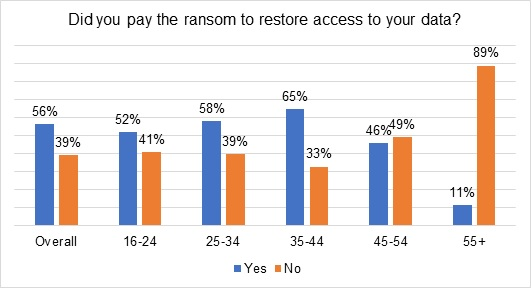
\includegraphics{images/ransom.jpg}
    \caption{\href{https://www.kaspersky.com/about/press-releases/over-half-of-ransomware-victims-pay-the-ransom-but-only-a-quarter-see-their-full-data-returned}{Segun una encuesta de Kaspersky}, más del 50\% de las victimas pagan el ransom, especialmente los usuarios más jovenes}
    \label{fig:ransom}
\end{figure}

\subsection{Tácticas y técnicas según MITRE ATT\&CK}
Según la matriz MITRE ATT\&CK para ICS, este ataque utilizó las siguientes tácticas y técnicas:

\begin{itemize}
    \item \textbf{Initial Access} - \textit{Spearphishing Attachment} (T0865), ya que el ataque comenzó cuando un empleado abrió un correo electrónico infectado.
    
    \item \textbf{Execution} - \textit{User Execution} (T0863), aprovechando el error humano para ejecutar código malicioso contenido en el correo electrónico.
    
    \item \textbf{Impact} - \textit{Data Encrypted for Impact} (T1486 of \textit{Enterprise} Matrix), el ransomware cifró datos críticos para exigir un rescate y paralizó las operaciones normales de la utilidad.\\
    Esto se puede relacionar con las técnicas de \textit{Loss of Control/Productivity and Revenue/Safety/Availability} (T0827, T0828, T0880 T0826).
\end{itemize}

\subsubsection{Justificación de las tácticas y técnicas}
Los atacantes eligieron estas tácticas por varias razones:

\begin{itemize}
    \item El phishing sigue siendo uno de los vectores de ataque más efectivos debido a su simplicidad y alta tasa de éxito, especialmente en organizaciones con personal no capacitado en seguridad cibernética.
    
    \item Las pequeñas municipalidades y servicios públicos suelen tener sistemas obsoletos y con parches de seguridad desactualizados, lo que las convierte en objetivos atractivos para ataques de ransomware.
    
    \item El cifrado de datos críticos para operaciones diarias crea una urgencia inmediata que aumenta la probabilidad de que la víctima pague el rescate.
    
    \item Los sistemas de control industrial conectados a redes administrativas permiten que un ataque que comienza en sistemas IT se propague a componentes OT críticos.
    
    \item Pueblos pequeños a menudo no tienen fondos suficiente para invertir en ciberseguridad, lo que los hace más vulnerables a ataques de ransomware.
    El hardware y software obsoleto, como el sistema de control de la utilidad de agua, a menudo carece de las actualizaciones de seguridad necesarias para resistir ataques modernos.
\end{itemize}



\subsection{Respuesta al incidente}
Pocos días después del ataque, el ayuntamiento votó unánimemente autorizar a su aseguradora a pagar 65 bitcoins, aproximadamente \$600,000, a los atacantes, más \$25,000 adicionales como deducible del seguro. A pesar del pago, los datos seguían siendo inaccesibles al 20 de junio de 2019, y no había garantía de recuperación completa.

Durante la recuperación, el departamento de IT logró restaurar parcialmente el sitio web de la ciudad y los servicios de correo electrónico. Las estaciones de bombeo de agua y los sistemas de prueba de calidad del agua se restablecieron solo parcialmente, requiriendo operaciones manuales para garantizar la continuidad del servicio.

Además del rescate, la ciudad autorizó gastar más de \$900,000 en nueva infraestructura informática, una inversión que estaba planificada para el año siguiente. Según un concejal, \ul{gran parte del hardware existente era antiguo y obsoleto}, lo que lo hacía vulnerable a ciberataques.

\subsubsection{Evaluación de la respuesta}
La respuesta al incidente presenta aspectos cuestionables:

\begin{itemize}
    \item Aunque es comprensible la decisión de pagar el rescate dado el impacto en servicios esenciales, esta acción, en general, incentiva futuros ataques.
    
    \item La inversión reactiva en nueva infraestructura demuestra que la ciudad reconoció la necesidad de modernización, pero lo hizo demasiado tarde, después de sufrir el ataque y pagar el rescate.
    
    \item La falta de actualizaciones y parches oportunos refleja una gestión de seguridad deficiente, especialmente considerando que estos sistemas controlaban infraestructura crítica.
\end{itemize}

Una respuesta más adecuada habría incluido:

\begin{itemize}
    \item Implementación continua y proactiva de un programa de actualización y aplicación de parches de seguridad.
    
    \item Formación regular en concienciación sobre ciberseguridad para todos los empleados, especialmente sobre la identificación de correos electrónicos de phishing.
    
    \item Segmentación efectiva entre redes IT y OT para evitar que un compromiso en sistemas administrativos afecte a los sistemas de control industrial.
    Este caso es un ejemplo claro de cómo la falta de segmentación y controles adecuados ha llevado al compromiso no solo de la utilidad de agua, sino de multiples oficinas gubernamentales, paralizando muchas operaciones de la ciudad.
    
    \item Desarrollo de un plan de continuidad de operaciones que permita la restauración rápida desde copias de seguridad sin necesidad de pagar rescates.
\end{itemize}

Este caso ilustra claramente cómo la falta de inversión en seguridad cibernética básica puede resultar en costos mucho mayores tras un incidente, incluyendo no solo el rescate y las nuevas adquisiciones, sino también daños reputacionales y pérdida de confianza pública.

\begin{paracol}{2}
    

    \colfill
    \begin{figure}[htbp]
        \centering
        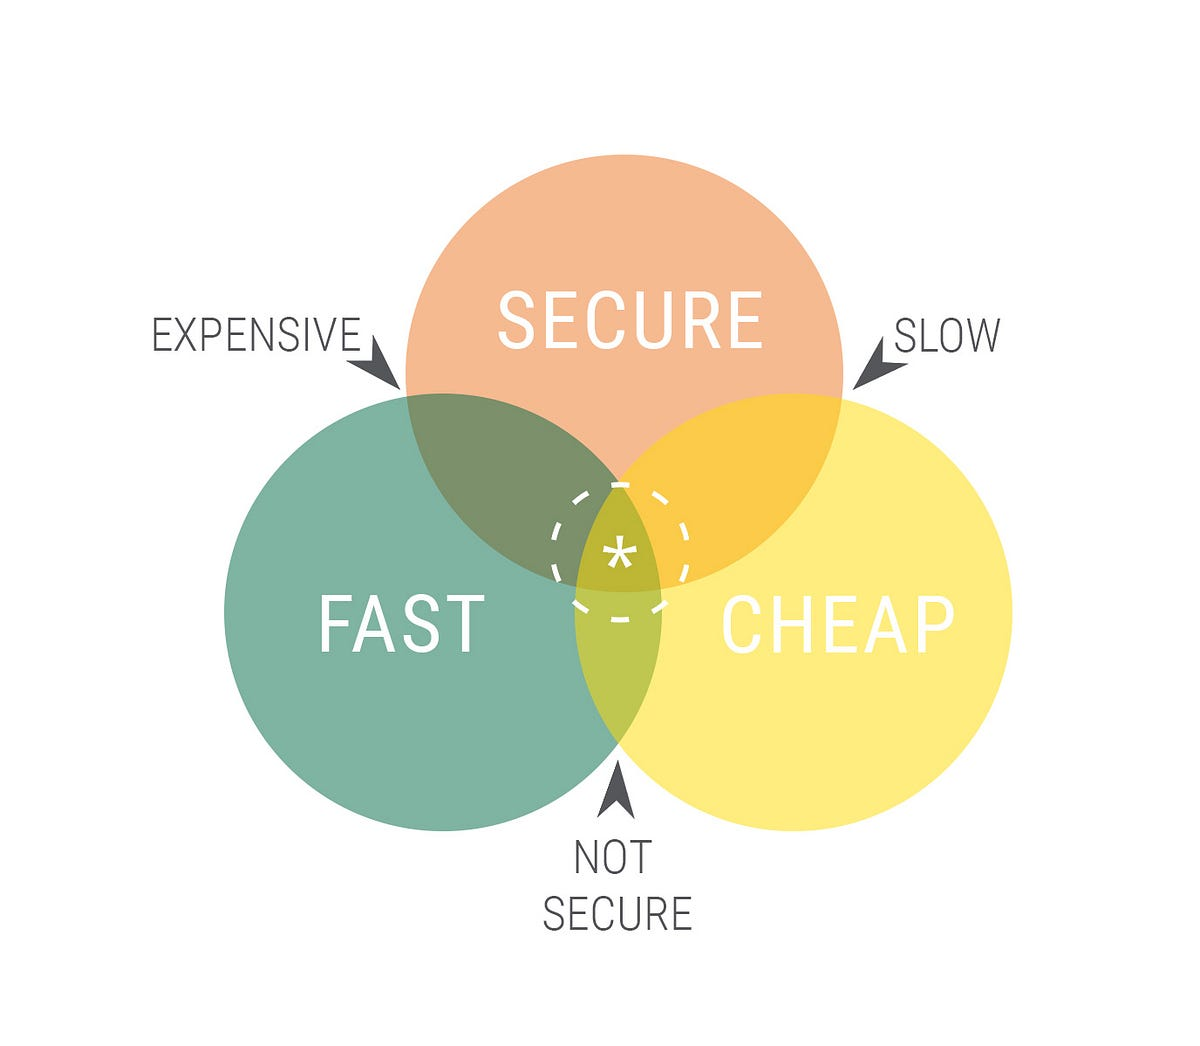
\includegraphics[width=0.85\columnwidth]{images/FSC.jpg}
        % \caption{}
        \label{fig:FSC}
    \end{figure}
    \colfill
    
    \switchcolumn
    Sin embargo, ilustra también cómo la seguridad sea un coste no indiferente, especialmente para pequeñas municipalidades que no tienen muchos recursos, y inversiones en ciberseguridad pueden ser vistas como un gasto innecesario.\\
    Claro que, típicamente el coste de un ataque exitoso es mucho mayor que el coste de una inversión en ciberseguridad, pero esto no es evidente para todos los responsables de la toma de decisiones, y para el público en general.
    
    Cómo un seguro de salud, o del coche, la ciberseguridad es una inversión que no se ve hasta que se necesita, y por lo tanto a menudo es minimizada o ignorada.\\
    Dado que ser robusto contra ciberataques puede ser difícil y costoso, debería haber al menos mecanismos de resistencia, que tienden a ser más baratos y fáciles de implementar, y que pueden ayudar a recuperarse ---casi--- fácilmente de un ataque sin pagar un rescate.
    
\end{paracol}


\newpage
\section{Ataque 5: Bowman Avenue Dam, EE.UU., 2013}

\begin{paracol}{2}
    
    \subsection{Descripción del incidente}

    \colfill
    En el año 2013, entre el 28 de agosto y el 18 de septiembre, hackers obtuvieron ``acceso remoto no autorizado'' al sistema SCADA de la presa Bowman Avenue en Rye, New York. Esta presa utiliza una compuerta controlada remotamente desde 2013 para controlar el flujo de agua según los niveles y temperaturas del arroyo Blind Brook. Los atacantes lograron recopilar información sobre niveles de agua, temperatura y estado de la compuerta, aunque esta estaba desconectada manualmente para mantenimiento durante la intrusión.

    El ataque se realizó mediante ``Google dorking'', una técnica que utiliza el motor de búsqueda Google para localizar vulnerabilidades en aplicaciones web. Los atacantes utilizaron comandos de búsqueda avanzada para identificar sistemas de control industrial expuestos en Internet, específicamente la aplicación web de monitoreo y control de la presa que carecía de medidas de seguridad básicas como firewall o autenticación.

    % \coolquote{
    %     This attack demonstrated how critical infrastructure systems can be discovered and compromised through simple reconnaissance techniques, highlighting the importance of implementing proper security controls before deploying internet-facing applications for industrial control systems.
    % }{}

    % El incidente marca uno de los primeros casos documentados de intrusión exitosa en infraestructura crítica estadounidense utilizando técnicas de reconocimiento de código abierto (OSINT). Aunque los atacantes no causaron daños físicos debido a que la compuerta estaba desconectada por mantenimiento, el acceso no autorizado demostró vulnerabilidades significativas en la seguridad de infraestructuras críticas conectadas a Internet.
    
    
    \colfill

    \switchcolumn

        \begin{figure}[htbp]
            \centering
            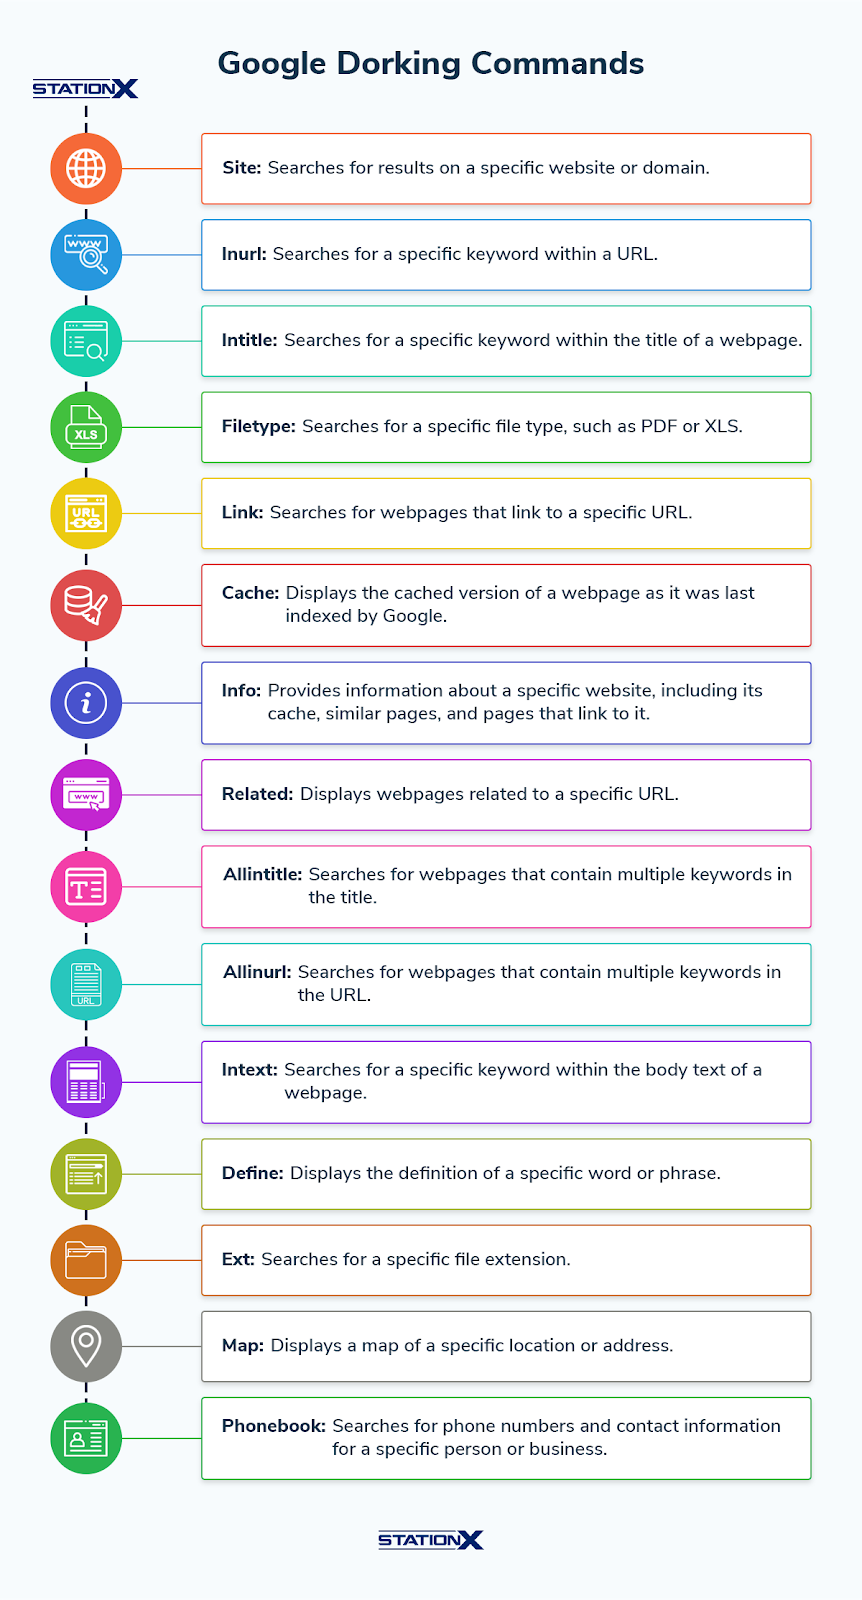
\includegraphics{images/googledorking.png}
            \caption{Google advanced search commands}
            \label{fig:googledorking}
        \end{figure}
    \end{paracol}
    
    \subsection{Tácticas y técnicas según MITRE ATT\&CK}
    Las tácticas y técnicas utilizadas incluyen:

\begin{itemize}
    \item \textbf{Reconnaissance} - \textit{Network Sniffing} (T0842) y \textit{Spoof Reporting Message} (T0856), utilizando Google dorking para identificar vulnerabilidades en la aplicación web de control de la presa.
    
    \item \textbf{Initial Access} - \textit{Exploit Public-Facing Application} (T0819), accediendo a la aplicación web de control sin protección adecuada.
    
    \item \textbf{Collection} - \textit{Automated Collection} (T0802), recopilando datos sobre niveles de agua, temperatura y estado de la compuerta.
\end{itemize}

\subsubsection{Justificación de las tácticas y técnicas}
Los atacantes eligieron estas tácticas porque:

\begin{itemize}
    \item El sistema de control estaba directamente accesible desde Internet sin firewall ni controles de autenticación, haciendo del reconocimiento una táctica efectiva.
        
        \item Google dorking es una técnica de bajo esfuerzo que permite identificar sistemas vulnerables sin alertar a los objetivos.
        
        \item La aplicación web para monitoreo y control no implementaba medidas de seguridad básicas, facilitando el acceso no autorizado.
        
        \item La recopilación de datos sobre el sistema proporcionaba información valiosa para posibles ataques futuros más destructivos.
        De hecho, se considera como el primer paso de la ``Cyber Kill Chain'' (CKC), que es un modelo que describe las etapas de un ciberataque, siendo las etapas posteriores el ataque real al sistema.
\end{itemize}

\newpage

\begin{figure}[htbp]
    \centering
    \includegraphics{images/bowmanDam.png}
    \caption{Bowman Avenue Dam}
    \label{fig:bowmanDam}
\end{figure}

\subsection{Respuesta al incidente}
Después del ataque, se instalaron un nuevo software y una nueva compuerta. Por dirección del Gobernador Cuomo, el Estado de Nueva York tomó múltiples medidas para mejorar sus capacidades de ciberseguridad en varios sectores. Las investigaciones realizadas por el DHS y el Departamento de Justicia resultaron en la acusación de varios hackers patrocinados por un estado. El ataque causó más de $30,000\$$ en costos de remediación.

\subsubsection{Evaluación de la respuesta}
La respuesta fue bastante adecuada.
La instalación de nuevo software y hardware con mejores características de seguridad es una medida importante para prevenir ataques basicos.\\
Además, es positivo que el ataque haya llevado al gobierno a tomar medidas para mejorar las capacidades de ciberseguridad a nivel estatal.



Algunas mejoras podrían ser:
\begin{itemize}
    % \item Implementación de evaluaciones de seguridad previas al despliegue de aplicaciones web críticas.
    \item Establecimiento de una arquitectura de acceso remoto seguro con múltiples capas de autenticación, posiblemente incluyendo información biométrica.
    \item Mejor segmentación de red para aislar sistemas críticos de control industrial de redes públicas y aplicaciones web.\\
    La compuerta de la presa estaba manualmente desconectada para mantenimiento durante la intrusión, por lo que los hackers no pudieron manipularla, pero esto fue simplemente suerte.
    \item Monitoreo continuo de búsquedas en Internet que puedan revelar información sensible sobre infraestructuras críticas, o vulnerabilidades en las aplicaciones utilizadas da dichas infraestructuras.
    % \item Implementación de programas de capacitación y concientización sobre ciberseguridad para el personal que gestiona infraestructuras críticas.
\end{itemize}

